\chapter{Teoretický úvod}
\label{sec:th}

% tcp/ip, osi k tomu asi dam jen citaci (ty knizky) do toho textu to tam je stejne zmineny jednou

\section{Názvosloví použité v~práci}

\begin{itemize}
    \item \textbf{Nadřazený systém} -- zařízení, jehož tvorba je cílem práce, je v~textu označováno jako nadřazený systém. Podrobná specifikace nadřazeného systému je popsána v~úvodu kapitoly \ref{sec:an}.
    \item \textbf{Podřízený systém} -- podřízené systémy jsou monitorovací zařízení, která jsou umístěná v~jednotlivých garážích. Zařízení neoperují samostatně, ale zasílají data nadřazenému systému. Podřízený systém je blíže popsán v~sekci \ref{sec:an_subsystem}.
    \item \textbf{Uživatel} -- uživatelem se v~textu práce myslí osoba spravující nadřazený systém a přistupující do jeho webového rozhraní. Jde tedy například o~majitele garáží nebo zaměstnance pověřeného jejich správou.
    \item \textbf{Klíč} -- náhodně generovaná data (například ve formě textového řetězce), která slouží k~ověření totožnosti. Znalost klíče umožní přístup k~šifrovaným datům nebo jinak zakázaným operacím. V~této práci se hovoří většinou o~API klíčích, kterými se prokazují podřízené systémy při komunikaci s~nadřazeným systémem.
    \item \textbf{Webové rozhraní} -- webovým rozhraním jsou v~textu práce myšleny webové stránky, pomocí kterých je možné spravovat nadřazený systém.
\end{itemize}

\section{Návrhový vzor MVC}

MVC (\textit{model-view-controller}) je návrhový vzor, který strukturuje aplikaci do tří částí \cite{mvc_dalling}:

\begin{itemize}
    \item \textit{Model} reprezentuje data v~aplikaci a operace, které s~nimi lze provádět. Důležitá vlastnost \textit{modelu} je nezávislost na \textit{view} a \textit{controlleru}. Díky tomu je možné stejný \textit{model} použít například pro webovou a nativní aplikaci.
    \item \textit{View} je zobrazení \textit{modelu} aplikace (například pomocí webových stránek).
    \item \textit{Controller} zpracovává uživatelský vstup a na jeho základě přenáší data mezi \textit{modelem} a \textit{view}.
\end{itemize}

Návrhový vzor MVC je použit při implementaci webové aplikace nadřazeného systému (bližší informace o~použití tohoto vzoru jsou v~sekci \ref{sec:de_mvc}).

\section{Protokol HTTP}

Při implementaci nadřazeného systému byl rozsáhle využit protokol HTTP (na tomto protokolu je postaveno uživatelské rozhraní a komunikace s~podřízenými systémy). Tato sekce popisuje s~ním spojené principy, které jsou zmiňovány v~dalším textu práce. 

\subsection{Model \textit{client/server}}

Protokol používá model \textit{client/server}. Klienti zasílají HTTP serveru požadavky, které server zpracovává a vytváří příslušné odpovědi \cite{tcp}. Spojení je tedy iniciováno na straně klienta a server pouze odpovídá. 

\subsection{Požadavek}

Požadavek (\textit{request}) zasílaný klientem tvoří následující části \cite{tcp}:

\begin{itemize}
    \item Metoda a URL zaslaného požadavku. V~této práci jsou použity především metody \texttt{get} a \texttt{post}. Metoda \texttt{get} slouží ke získávání dat (například HTML stránek) ze serveru. Metoda \texttt{post} je určená k~zasílání nových informací serveru.
    \item Záhlaví obsahující jednotlivé hlavičky požadavku. Tato část je v~práci využita pro zaslání API klíče podřízeného systému, viz sekci \ref{sec:de_api}.
    \item Volitelná přenášená data (například obsah HTML formuláře).
\end{itemize}

Na požadavek server odpovídá zasláním požadovaných dat (pokud jsou dostupná) a návratovým kódem, který indikuje úspěšnost dotazu \cite{tcp}.

% \subsection{Relace}

\subsection{Rozšíření HTTPS}

Samotný protokol HTTP neimplementuje žádné šifrování, proto vzniklo jeho rozšíření zabezpečené protokolem SSL či TLS\footnote{Dále je pro jednoduchost zmiňován jen protokol TLS podle normy RFC-5246 \cite{rfc5246}.}, nazvané HTTPS \cite{tcp_sec}.

Protokol TLS umožňuje autentizaci serveru pomocí certifikátu (viz sekci \ref{sec:th_cert}) a domluvu serveru a klienta na společném klíči \cite{tcp_sec}. Tímto klíčem je pak šifrována veškerá komunikace mezi klientem a serverem \cite{tcp_sec}.

%\section{Protokol MQTT} 

% napsat ze pro sifrovani taky pouziva tls

% \subsection{Model \textit{publisher/subscriber}}

% \section{Cloud}

% \section{API} to mozna necham jen ve zkratkach, stejne tak JSON

% \section{Vícevláknová obsluha} ????

\section{Certifikát}
\label{sec:th_cert}

Certifikát je obecně struktura sloužící k~ověření totožnosti účastníka komunikace a distribuci jeho veřejného klíče \cite{tcp_sec}. V~této práci se certifikátem myslí certifikát podle normy X.509 \cite{rfc2459}, který je používán protokolem TLS \cite{rfc5246}.

\subsection{Certifikační autorita}

Certifikační autorita je subjekt, který se zabývá vydáváním certifikátů. Teoreticky může certifikát vydat kdokoliv, k~ověření totožnosti serveru lze však použít pouze certifikát vydaný důvěryhodnou certifikační autoritou.

U~takového certifikátu lze ověřit jeho pravost a tím zaručit, že nebyl podvržen (útok založený na podvrženém certifikátu popisuje sekce \ref{sec:th_mitm}) \cite{tcp_sec}.

Využití certifikátů v~rámci této práce je blíže popsáno v~sekci \ref{sec:an_certs}.

\section{CSRF -- \textit{Cross-site request forgery}}

CSRF je forma útoku na webovou aplikaci, při kterém může útočník odeslíat falešné požadavky pomocí prohlížeče přihlášeného uživatele \cite{csrf_owasp}. Útok může mít následující průběh:

\begin{enumerate}
    \item Uživatel je v~jedné záložce prohlížeče prihlášen do svého internetového bankovnictví, které není zabezpečeno proti CSRF.
    \item Útočník pošle uživateli odkaz na stránku, na který uživatel klikne.
    \item Stránka po načtení zašle požadavek internetovému bankovnictí, potvrzující převod peněz na útočníkův účet. Tento požadavek je platný, neboť pochází z~prohlížeče přihlášeného uživatele. 

    Nezabezpečená aplikace internetového bankovnictví nemá jak ověřit, že požadavek nepřišel z~jejich stránek.
\end{enumerate}

Útok se dá použít k~zaslání nežádoucího požadavku (v~kontextu této práce například na smazání záznamu o~garáži), ne však ke získání dat ze stránky \cite{csrf_owasp}. Tomu zabraňuje koncept nazvaný \textit{same origin policy}, implementovaný v~současných prohlížečích \cite{sec_handbook}. Tento koncept omezuje to, jak spolu mohou inter\-agovat webové stránky na různých doménách.

Ochranu proti CSRF je možné implementovat vkládáním náhodně generovaných \textit{tokenů} do formulářů na webové stránce. Při odeslání formuláře se pak původ požadavku ověří pomocí tohoto \textit{tokenu} -- zaslaný \textit{token} se musí shodovat s~\textit{tokenem} vloženým ve webové stránce.

Přihlášený uživatel má přístup k~webovým stránkám aplikace, a je tedy možné do odeslaného požadavku vložit ověřovací \textit{token} získaný z~formuláře. 

Naopak útočník může pouze zasílat požadavky, ale ne získávat data ze stránek, a tudíž nemá přístup k~\textit{tokenu}, kterým by mohl svůj požadavek zfalšovat.

Zde je opět důležitá \textit{same origin policy}, která získání \textit{tokenu} zabraňuje. Pokud by tento mechanismus nefungoval, mohl by útočník kromě zasílání požadavků také získávat data ze stránky, a tedy i platné \textit{tokeny}.

Webová aplikace implementovaná v~této práci využívá právě tento způsob ochrany proti CSRF (více v~sekci \ref{sec:im_controller}).

\section{\textit{Attack surface}}

\textit{Attack surface} popisuje všechny možné body, kde by mohl potencionální útočník napadnout daný systém \cite{attack_surface_owasp}. V~práci je zmíněn v~sekci \ref{sec:an_cloud}, ve spojitosti se zvýšeným ohrožením při provozu serveru dostupného z~internetu.

\section{\textit{Man-in-the-middle} útok}
\label{sec:th_mitm}

\textit{Man-in-the-middle} útok na protokolu HTTPS využívá situace, kdy certifikát pro ověření totožnosti serveru není důvěryhodný a může být zfalšován \cite{mitm}. Schéma útoku popisuje obrázek \ref{fig:mitm}. 

V~tom případě může útočník (\textcolor{magenta}{Eva}) zachytit komunikaci mezi klientem (\textcolor{green}{Bob}) a serverem (\textcolor{blue2}{Alice}), a místo certifikátu serveru zaslat klientovi svůj certifikát. Poté je komunikace rozdělena na dvě části \cite{mitm}:

\begin{enumerate}
    \item \textcolor{green}{Bob} komunikuje s~\textcolor{magenta}{Evou} jako by to byla \textcolor{blue2}{Alice}. K~této komunikaci má \textcolor{magenta}{Eva} úplný přístup, neboť je šifrována pomocí jejího certifikátu.
    \item Po zachycení komunikace od \textcolor{green}{Boba} \textcolor{magenta}{Eva} tyto data přepošle \textcolor{blue2}{Alici}. \textcolor{blue2}{Alice} zašle \textcolor{magenta}{Evě} odpověď šifrovanou pomocí původního certifikátu. \textcolor{magenta}{Eva} tuto odpověď přečte, opět zašifruje pomocí svého certifikátu a pošle \textcolor{green}{Bobovi}.
\end{enumerate}

V~tomto scénáři \textcolor{green}{Bob} netuší, že nekomunikuje s~\textcolor{blue2}{Alicí}. Jelikož \textcolor{blue2}{Alice} nedodala důvěryhodný certifikát, nemůže \textcolor{green}{Bob} zjistit, že používá zfalšovaný.

\begin{figure}[h!]
    \centering
    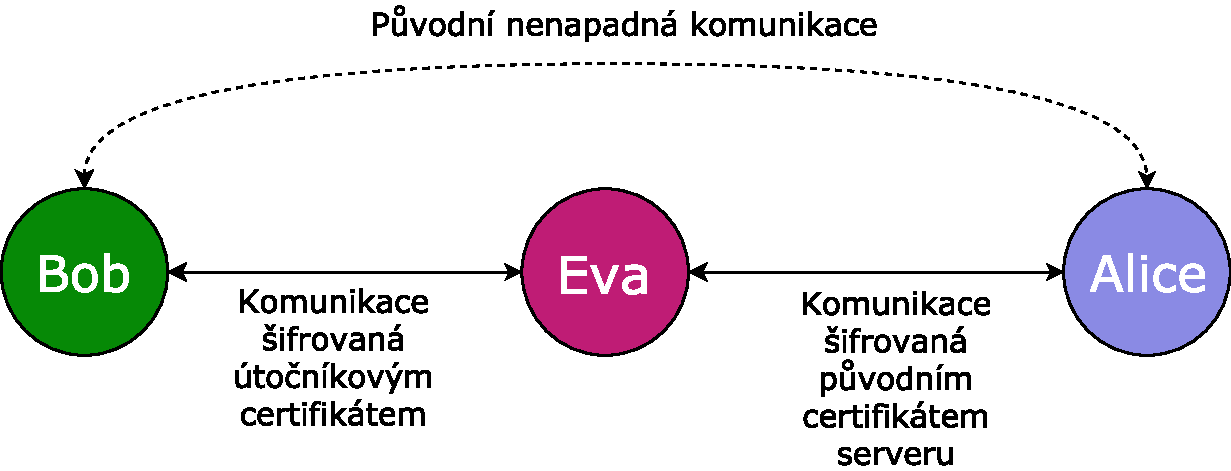
\includegraphics[width=\textwidth]{images/mitm.pdf}
    \caption[\textit{Man-in-the-middle} útok]{\textit{Man-in-the-middle} útok. Eva funguje jako nežádoucí prostředník mezi Bobem (klientem) a Alicí (původním serverem). Díky tomu má přístup ke zprávám obou účastníků komunikace. \cite{mitm}}
    \label{fig:mitm}
\end{figure}

V~textu práce je možnost \textit{man-in-the-middle} útoku diskutována v~části zabývající se volbou certifikátu pro provoz HTTPS (sekce \ref{sec:an_certs}).

\section{\textit{Hashování}}

\textit{Hashováním} se obecně rozumí vytvoření otistku pevné délky -- \textit{hashe} -- z~libovolných vstupních dat. Důležitou vlastností je jednosměrnost tohoto procesu, tedy že z~vytvořeného otisku již nelze (v~rozumném čase) zrekonstruovat původní vstup. \cite{hash_crackstation}

\textit{Hashování} se používá k~zabezpeční uložených hesel. Heslo uložené v~čitelné podobě není při úniku souboru s~heslem nijak chráněno. Proto je vhodné uložit místo hesla samotného jeho \textit{hash}. Pokud dojde k~úniku \textit{hashovaných} hesel, je pro útočníka velmi problematické získat z~otisků čitelná hesla \cite{hash_crackstation}.

\textit{Hashování} lze provést pomocí mnoha algortimů, ne všechny se však hodí k~zabezpečení ukládaných hesel. Některé algoritmy, jako například MD5 či SHA-1, nejsou dostatečně výpočetně náročné, takže umožňují efektivní útoky hrubou silou (lze dostatečně rychle spočítat všechny možné kombinace vstupů do dané délky, a tím zjistit jaký vstup odpovídá danému \textit{hashi}) \cite{hash_crackstation}. 

Pro bezpečné ukládání hesel je nutné použít dostatečné náročný algoritmus. V~této práci je použit algoritmus Argon2, který je považován za vhodný k~\textit{hashování} uložených hesel \cite{hash_crackstation}.

\subsection{Solení \textit{hashů}}

\textit{Hashování} hesla je vhodné doplnit o~proces takzvaného \uv{solení}. Při něm se nevytváří otisk samotného hesla, ale hesla doplněného o~náhodně vygenerovaný řetězec -- sůl. To ztěžuje použítí předpočítaných tabulek (například tabulky s~otisky často používaných hesel) pro útoky hrubou silou \cite{hash_crackstation}.

Pro bližší informace o~bezpečném ukládání hesel doporučuji článek \textit{Salted Password Hashing - Doing it Right} \cite{hash_crackstation}.
